\documentclass[11pt,a4paper]{article}
% Preambulo comun de los reportes de Tecnologias Celulares.
% Cada main.tex hace: \documentclass ... % Preambulo comun de los reportes de Tecnologias Celulares.
% Cada main.tex hace: \documentclass ... % Preambulo comun de los reportes de Tecnologias Celulares.
% Cada main.tex hace: \documentclass ... \input{../comun/preambulo.tex}
\usepackage[utf8]{inputenc}
\usepackage[T1]{fontenc}
\usepackage[spanish,mexico]{babel}
\usepackage{graphicx}
\usepackage[margin=2.5cm]{geometry}
\usepackage{amsmath}
\usepackage{amssymb}
\usepackage{booktabs}
\usepackage{tabularx}
\usepackage{array}
\usepackage{float}
\usepackage{setspace}
\usepackage{parskip}
\usepackage{fancyhdr}
\usepackage{textcomp}
\usepackage{xcolor}
\usepackage{caption}
\usepackage{fvextra}
\usepackage[hidelinks]{hyperref}

\onehalfspacing
\setlength{\parskip}{6pt}
\sloppy
\setlength{\emergencystretch}{3em}
\setlength{\headheight}{40pt}
\captionsetup{font=small,labelfont=bf}
\setlength{\tabcolsep}{6pt}

\pagestyle{fancy}
\fancyhf{}
\fancyhead[L]{\includegraphics[width=1cm]{/home/yovick/repos/UAZ-IEI/Assets/UIE.png}}
\fancyhead[R]{\small Comunicaciones Inalámbricas}
\fancyfoot[C]{\thepage}
\renewcommand{\headrulewidth}{0.4pt}

\DefineVerbatimEnvironment{codigo}{Verbatim}{%
  breaklines=true,breakanywhere=true,fontsize=\small,frame=single,
  framesep=3pt,rulecolor=\color{gray!50}}

% Figura centrada con pie: \figura[ancho]{archivo}{leyenda}
\newcommand{\figura}[3][0.85]{%
  \begin{center}
    \includegraphics[width=#1\linewidth]{#2}\\[2pt]
    {\small #3}
  \end{center}}

% Portada: \portada{numero}{titulo de la practica}
\newcommand{\portada}[2]{%
\begin{titlepage}
  \thispagestyle{empty}
  \begin{center}
    \vspace*{1cm}
    \includegraphics[width=4.5cm]{/home/yovick/repos/UAZ-IEI/Assets/uaz.png}
    \vspace{0.8cm}

    {\large Universidad Autónoma de Zacatecas}\\[4pt]
    {\large Unidad Académica de Ingeniería Eléctrica}\\[4pt]
    {\normalsize Ingeniería Electrónica Industrial con especialidad en Telecomunicaciones}

    \vspace{1.8cm}
    {\LARGE\bfseries Práctica #1}\\[10pt]
    {\Large\bfseries #2}
  \end{center}

  \vspace{2.2cm}
  \begin{center}
    \begin{tabular}{rl}
      \textbf{Materia:} & Comunicaciones Inalámbricas\\
      \textbf{Docente:} & Dr. Víktor Iván Rodríguez Abdalá\\
      \textbf{Alumno:}  & Arnold Yovick Ríos Zaldívar\\
      \textbf{Fecha:}   & Noviembre de 2026\\
    \end{tabular}
  \end{center}
  \vfill
\end{titlepage}}

\usepackage[utf8]{inputenc}
\usepackage[T1]{fontenc}
\usepackage[spanish,mexico]{babel}
\usepackage{graphicx}
\usepackage[margin=2.5cm]{geometry}
\usepackage{amsmath}
\usepackage{amssymb}
\usepackage{booktabs}
\usepackage{tabularx}
\usepackage{array}
\usepackage{float}
\usepackage{setspace}
\usepackage{parskip}
\usepackage{fancyhdr}
\usepackage{textcomp}
\usepackage{xcolor}
\usepackage{caption}
\usepackage{fvextra}
\usepackage[hidelinks]{hyperref}

\onehalfspacing
\setlength{\parskip}{6pt}
\sloppy
\setlength{\emergencystretch}{3em}
\setlength{\headheight}{40pt}
\captionsetup{font=small,labelfont=bf}
\setlength{\tabcolsep}{6pt}

\pagestyle{fancy}
\fancyhf{}
\fancyhead[L]{\includegraphics[width=1cm]{/home/yovick/repos/UAZ-IEI/Assets/UIE.png}}
\fancyhead[R]{\small Comunicaciones Inalámbricas}
\fancyfoot[C]{\thepage}
\renewcommand{\headrulewidth}{0.4pt}

\DefineVerbatimEnvironment{codigo}{Verbatim}{%
  breaklines=true,breakanywhere=true,fontsize=\small,frame=single,
  framesep=3pt,rulecolor=\color{gray!50}}

% Figura centrada con pie: \figura[ancho]{archivo}{leyenda}
\newcommand{\figura}[3][0.85]{%
  \begin{center}
    \includegraphics[width=#1\linewidth]{#2}\\[2pt]
    {\small #3}
  \end{center}}

% Portada: \portada{numero}{titulo de la practica}
\newcommand{\portada}[2]{%
\begin{titlepage}
  \thispagestyle{empty}
  \begin{center}
    \vspace*{1cm}
    \includegraphics[width=4.5cm]{/home/yovick/repos/UAZ-IEI/Assets/uaz.png}
    \vspace{0.8cm}

    {\large Universidad Autónoma de Zacatecas}\\[4pt]
    {\large Unidad Académica de Ingeniería Eléctrica}\\[4pt]
    {\normalsize Ingeniería Electrónica Industrial con especialidad en Telecomunicaciones}

    \vspace{1.8cm}
    {\LARGE\bfseries Práctica #1}\\[10pt]
    {\Large\bfseries #2}
  \end{center}

  \vspace{2.2cm}
  \begin{center}
    \begin{tabular}{rl}
      \textbf{Materia:} & Comunicaciones Inalámbricas\\
      \textbf{Docente:} & Dr. Víktor Iván Rodríguez Abdalá\\
      \textbf{Alumno:}  & Arnold Yovick Ríos Zaldívar\\
      \textbf{Fecha:}   & Noviembre de 2026\\
    \end{tabular}
  \end{center}
  \vfill
\end{titlepage}}

\usepackage[utf8]{inputenc}
\usepackage[T1]{fontenc}
\usepackage[spanish,mexico]{babel}
\usepackage{graphicx}
\usepackage[margin=2.5cm]{geometry}
\usepackage{amsmath}
\usepackage{amssymb}
\usepackage{booktabs}
\usepackage{tabularx}
\usepackage{array}
\usepackage{float}
\usepackage{setspace}
\usepackage{parskip}
\usepackage{fancyhdr}
\usepackage{textcomp}
\usepackage{xcolor}
\usepackage{caption}
\usepackage{fvextra}
\usepackage[hidelinks]{hyperref}

\onehalfspacing
\setlength{\parskip}{6pt}
\sloppy
\setlength{\emergencystretch}{3em}
\setlength{\headheight}{40pt}
\captionsetup{font=small,labelfont=bf}
\setlength{\tabcolsep}{6pt}

\pagestyle{fancy}
\fancyhf{}
\fancyhead[L]{\includegraphics[width=1cm]{/home/yovick/repos/UAZ-IEI/Assets/UIE.png}}
\fancyhead[R]{\small Comunicaciones Inalámbricas}
\fancyfoot[C]{\thepage}
\renewcommand{\headrulewidth}{0.4pt}

\DefineVerbatimEnvironment{codigo}{Verbatim}{%
  breaklines=true,breakanywhere=true,fontsize=\small,frame=single,
  framesep=3pt,rulecolor=\color{gray!50}}

% Figura centrada con pie: \figura[ancho]{archivo}{leyenda}
\newcommand{\figura}[3][0.85]{%
  \begin{center}
    \includegraphics[width=#1\linewidth]{#2}\\[2pt]
    {\small #3}
  \end{center}}

% Portada: \portada{numero}{titulo de la practica}
\newcommand{\portada}[2]{%
\begin{titlepage}
  \thispagestyle{empty}
  \begin{center}
    \vspace*{1cm}
    \includegraphics[width=4.5cm]{/home/yovick/repos/UAZ-IEI/Assets/uaz.png}
    \vspace{0.8cm}

    {\large Universidad Autónoma de Zacatecas}\\[4pt]
    {\large Unidad Académica de Ingeniería Eléctrica}\\[4pt]
    {\normalsize Ingeniería Electrónica Industrial con especialidad en Telecomunicaciones}

    \vspace{1.8cm}
    {\LARGE\bfseries Práctica #1}\\[10pt]
    {\Large\bfseries #2}
  \end{center}

  \vspace{2.2cm}
  \begin{center}
    \begin{tabular}{rl}
      \textbf{Materia:} & Comunicaciones Inalámbricas\\
      \textbf{Docente:} & Dr. Víktor Iván Rodríguez Abdalá\\
      \textbf{Alumno:}  & Arnold Yovick Ríos Zaldívar\\
      \textbf{Fecha:}   & Noviembre de 2026\\
    \end{tabular}
  \end{center}
  \vfill
\end{titlepage}}


\graphicspath{{figs/}}

\begin{document}
\thispagestyle{empty}

% --------------------------------------------------------------- encabezado
\begin{center}
  \includegraphics[width=2.6cm]{/home/yovick/repos/UAZ-IEI/Assets/uaz.png}\\[2mm]
  {\large Universidad Autónoma de Zacatecas}\\
  {\normalsize Unidad Académica de Ingeniería Eléctrica}\\
  {\normalsize Ingeniería Electrónica Industrial con especialidad en Telecomunicaciones}\\[6mm]
  {\LARGE\bfseries Tarea 2}\\[2mm]
  {\large Capacidad de canal, códigos y decodificación}\\[5mm]
  {\small
  \begin{tabular}{rl}
    \textbf{Materia:}   & Comunicaciones Inalámbricas\\
    \textbf{Docente:}   & Dr. Víktor Iván Rodríguez Abdalá\\
    \textbf{Alumno:}    & Arnold Yovick Ríos Zaldívar\\
    \textbf{Matrícula:} & 35167151 \quad \textbf{Grupo:} VII\\
    \textbf{Fecha:}     & Noviembre de 2026\\
  \end{tabular}}
\end{center}

\vspace{2mm}

Los 26 problemas se resolvieron con \texttt{tarea2.py}. El script genera las
figuras en \texttt{figs/}, los números en \texttt{datos/resultados.json} y
abre las ventanas de las figuras al terminar. Todas las gráficas usan el estilo
oscuro del repositorio.

\textbf{Supuestos.} El PDF de la tarea remite a los problemas ilustrativos 3,
10, 12 y 22, a la Figura 18 y a la Ecuación (80) de las notas del curso, que no
vienen incluidas en el documento. Se usaron las convenciones estándar de un
curso de comunicaciones: la Figura 18 es el codificador convolucional de tasa
$1/2$ con generadores $(5,7)$ en octal y $K=3$; el problema ilustrativo 10 es el
código de Hamming $(7,4)$ con decisión dura; el 12 es su extensión a decisión
suave; el 22 es un turbo código con constituyentes RSC $(5,7)$, modulación BPSK
y canal AWGN; y la Ecuación (80) reúne las identidades de \emph{log-sum-exp} y
de la LLR del XOR. Si el curso usa otra numeración, los resultados numéricos
cambian, pero el procedimiento es el mismo.

% =======================================================================
\section*{1. Capacidad de canal (problemas 1 a 9)}

\subsection*{Problema 1: capacidad del canal simétrico binario}

Para un canal simétrico binario (BSC) con probabilidad de cruce $p$,
\begin{equation}
  C(p)=1-H_b(p),\qquad
  H_b(p)=-p\log_2 p-(1-p)\log_2(1-p).
\end{equation}
La capacidad se anula en $p=1/2$, donde la salida no dice nada de la entrada,
y vale 1 en $p=0$ y $p=1$ (en $p=1$ el canal es un inversor determinista). Los
valores calculados son $C(0.1)=0.5310$ y $C(0.25)=0.1887$.
\begin{figure}[H]
  \centering
  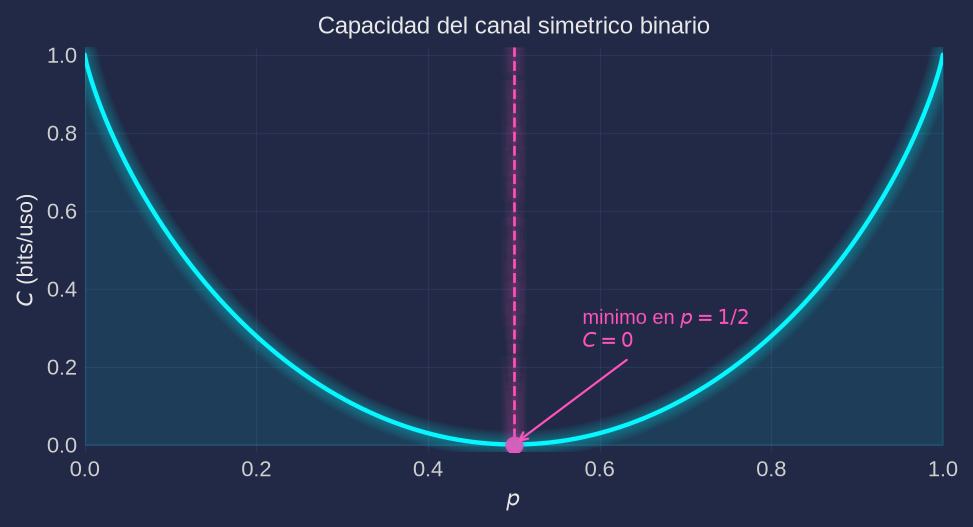
\includegraphics[width=0.82\linewidth]{p01_bsc.png}
  \caption{Capacidad del BSC. El mínimo es $C=0$ en $p=1/2$.}
\end{figure}

\subsection*{Problema 2: canal binario no simétrico}

Con $p(0|1)=0.2$ y $p(1|0)=0.4$, la matriz del canal es
\begin{equation}
  P(Y|X)=
  \begin{pmatrix}
    0.6 & 0.4\\
    0.2 & 0.8
  \end{pmatrix}.
\end{equation}
Para $p=P(X=1)$,
\begin{equation}
  P(Y=0)=0.6-0.4p,\qquad
  I(X:Y)=H_b(0.6-0.4p)-(1-p)H_b(0.4)-pH_b(0.2).
\end{equation}
Maximizando numéricamente, $p^*=0.5156$ e $I_{\max}=0.1246$ bits. El máximo no
está en $p=1/2$ porque el canal es asimétrico.
\begin{figure}[H]
  \centering
  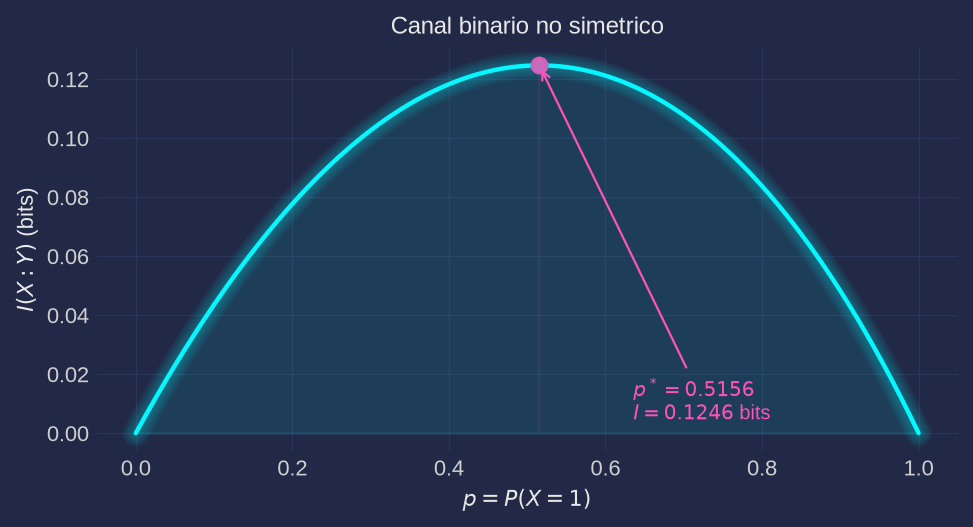
\includegraphics[width=0.82\linewidth]{p02_no_simetrico.png}
  \caption{Información mutua del canal no simétrico contra $p=P(X=1)$.}
\end{figure}

\subsection*{Problema 3: canal Z}

En el canal Z, $p(0|1)=\epsilon$ y $p(1|0)=0$. Para $p=P(X=1)$,
\begin{equation}
  P(Y=0)=1-p(1-\epsilon),\qquad
  I(X:Y)=H_b\!\left(1-p(1-\epsilon)\right)-pH_b(\epsilon).
\end{equation}
La tabla siguiente contiene la capacidad numérica para cada $\epsilon$. Para
$\epsilon=0$ el canal es transparente y $C=1$; para $\epsilon=1$ ambas
entradas producen siempre 0 y $C=0$. Cuando $\epsilon$ crece, la capacidad baja
y la distribución óptima se aleja de $p=1/2$.
\begin{table}[H]
  \centering
  \begin{tabular}{cccccccccc}
    \toprule
    $\epsilon$ & 0 & 0.1 & 0.2 & 0.3 & 0.4 & 0.5 & 0.7 & 0.9 & 1\\
    \midrule
    $C$ & 1 & 0.7628 & 0.6182 & 0.5037 & 0.4068 & 0.3219 & 0.1770 & 0.0548 & 0\\
    $p^*$ & 0.5 & 0.4563 & 0.4357 & 0.4210 & 0.4095 & 0.4000 & 0.3848 & 0.3730 & --\\
    \bottomrule
  \end{tabular}
  \caption{Capacidad del canal Z y distribución óptima.}
\end{table}
\begin{figure}[H]
  \centering
  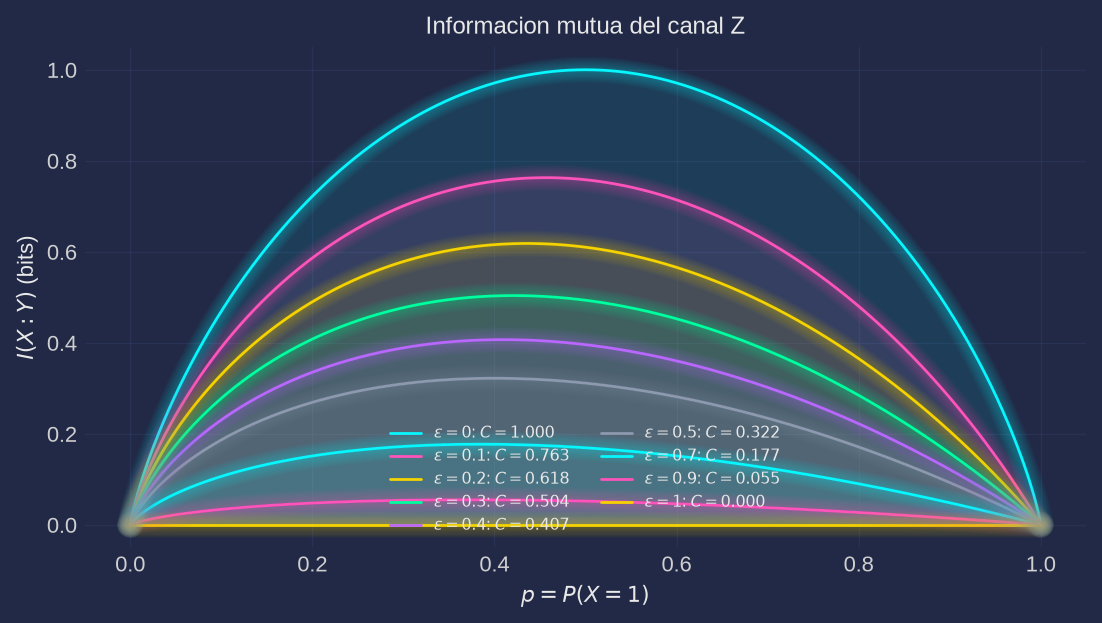
\includegraphics[width=0.9\linewidth]{p03_z.png}
  \caption{Información mutua del canal Z para varios valores de $\epsilon$.}
\end{figure}

\subsection*{Problema 4: entrada binaria y salida ternaria}

Las probabilidades que faltan se obtienen porque cada renglón suma uno:
\begin{equation}
  P(Y|X)=
  \begin{pmatrix}
    0.05 & 0.20 & 0.75\\
    0.10 & 0.10 & 0.80
  \end{pmatrix}.
\end{equation}
Maximizando $I(X:Y)$ se obtiene $p^*=0.5092$ y $C=0.01897$ bits. La capacidad
es muy baja porque las dos entradas producen casi siempre el símbolo 2: la
salida contiene poca información sobre la entrada.
\begin{figure}[H]
  \centering
  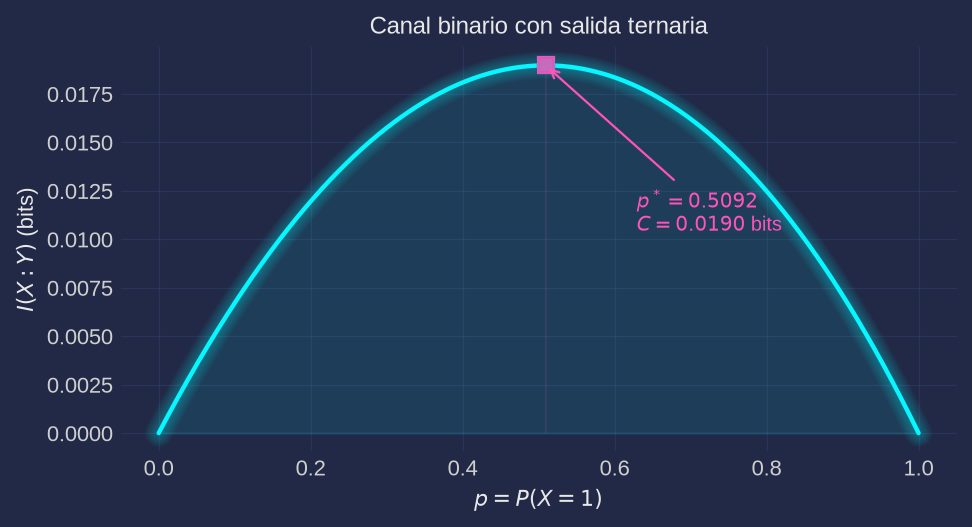
\includegraphics[width=0.82\linewidth]{p04_binario_ternario.png}
  \caption{Canal binario con salida ternaria.}
\end{figure}

\subsection*{Problema 5: entrada ternaria y salida binaria}

Con $p(0|0)=0.05$, $p(1|1)=0.2$ y $p(0|2)=0.1$, la matriz completa es
\begin{equation}
  P(Y|X)=
  \begin{pmatrix}
    0.05 & 0.95\\
    0.80 & 0.20\\
    0.10 & 0.90
  \end{pmatrix}.
\end{equation}
La capacidad se maximiza sobre el símplex $p_0+p_1+p_2=1$. El resultado es
$p_0^*=0.5324$, $p_1^*=0.4676$, $p_2^*=0$ y $C=0.4813$ bits. La entrada 2 no
se usa porque su salida es casi siempre 1, igual que la de la entrada 0, y no
aporta información nueva.
\begin{figure}[H]
  \centering
  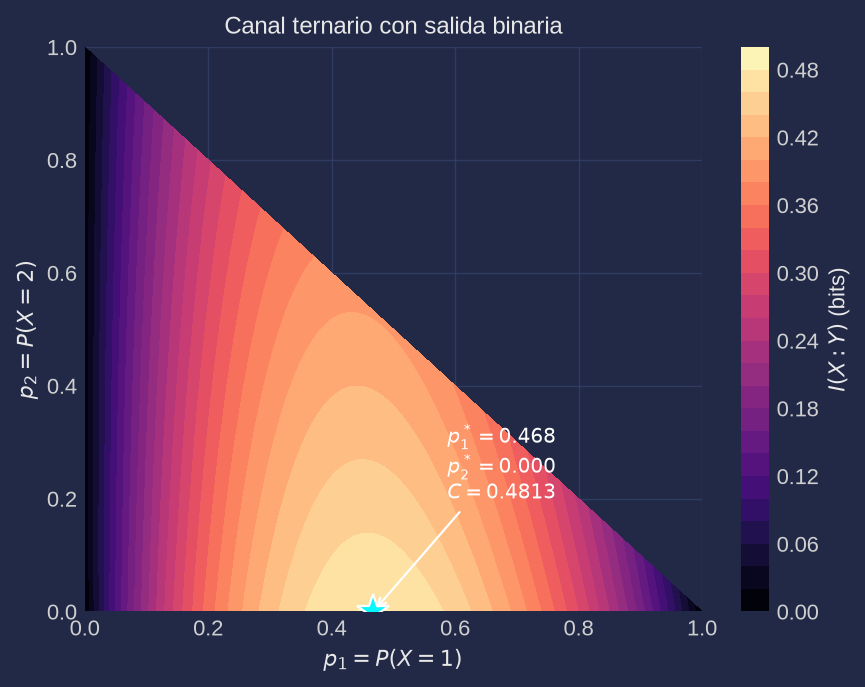
\includegraphics[width=0.62\linewidth]{p05_ternario_binario.png}
  \caption{Información mutua del canal ternario-binario sobre el símplex.}
\end{figure}

\subsection*{Problema 6: BSC con señalización ortogonal binaria}

Para señales ortogonales binarias con detección coherente,
$P_e=Q(\sqrt{E_b/N_0})$ y el canal equivalente es un BSC con esa probabilidad
de cruce. Por tanto,
\begin{equation}
  C=1-H_b\!\left(Q\!\left(\sqrt{E_b/N_0}\right)\right).
\end{equation}
Los valores son $C(0\,\text{dB})=0.3689$, $C(6\,\text{dB})=0.8420$ y
$C(10\,\text{dB})=0.9908$.
\begin{figure}[H]
  \centering
  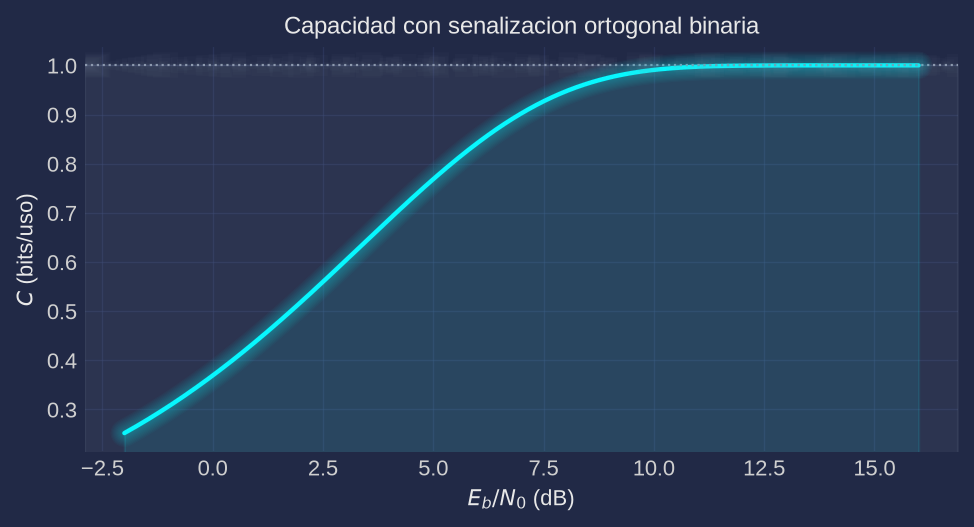
\includegraphics[width=0.82\linewidth]{p06_ortogonal.png}
  \caption{Capacidad del BSC equivalente a señalización ortogonal binaria.}
\end{figure}

\subsection*{Problema 7: señales ortogonales contra antipodales}

Si las dos señales tienen la misma energía, las antipodales tienen distancia
$2\sqrt{E_b}$ y las ortogonales $\sqrt{2E_b}$. Por eso
\begin{equation}
  P_{e,\text{ant}}=Q\!\left(\sqrt{\frac{2E_b}{N_0}}\right),\qquad
  P_{e,\text{ort}}=Q\!\left(\sqrt{\frac{E_b}{N_0}}\right).
\end{equation}
La curva de capacidad de las ortogonales queda 3 dB a la derecha. Para
$C=0.5$, las antipodales necesitan $-1.24$ dB y las ortogonales $1.79$ dB; la
penalización es $3.03$ dB. En el límite de $E_b/N_0\to\infty$ ambas capacidades
tienden a 1, pero a baja SNR la ortogonal es claramente peor.
\begin{figure}[H]
  \centering
  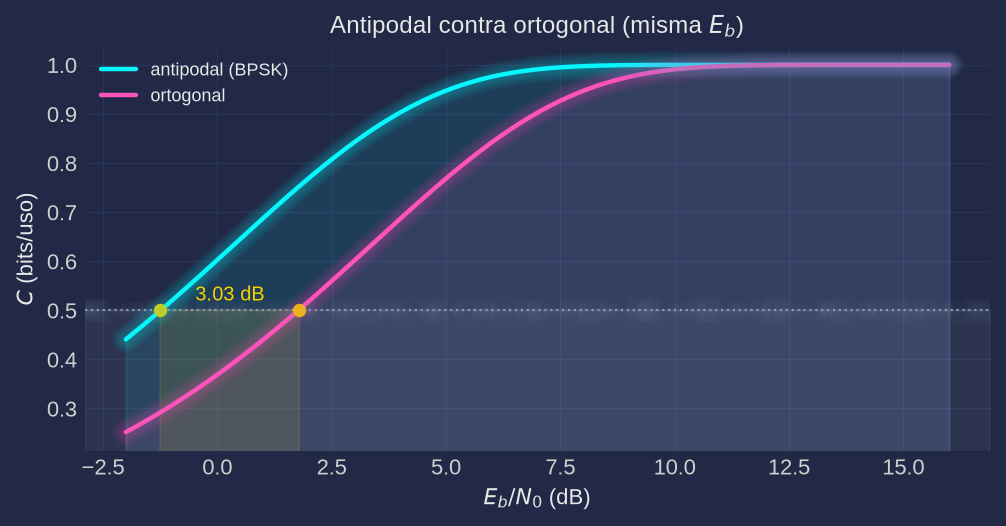
\includegraphics[width=0.85\linewidth]{p07_antipodal_ortogonal.png}
  \caption{Capacidad de señalización antipodal y ortogonal con la misma $E_b$.}
\end{figure}

\subsection*{Problema 8: decisión dura contra decisión suave}

En decisión dura se cuantiza la salida a un bit y se usa un BSC con
$P_e=Q(\sqrt{2E_b/N_0})$ para antipodal o $Q(\sqrt{E_b/N_0})$ para ortogonal.
En decisión suave se conserva la salida analógica. Para entrada binaria
equiprobable y LLR $L=\log[p(y|0)/p(y|1)]$,
\begin{equation}
  C=1-\mathbb{E}\!\left[\log_2(1+e^{-L})\right].
\end{equation}
Con BPSK, $L|0\sim\mathcal{N}(4\gamma,8\gamma)$ para antipodal y
$L|0\sim\mathcal{N}(2\gamma,4\gamma)$ para ortogonal, con $\gamma=E_b/N_0$.
A 6 dB se obtiene:
\begin{table}[H]
  \centering
  \begin{tabular}{lcc}
    \toprule
    Señalización & Decisión dura & Decisión suave\\
    \midrule
    Ortogonal & 0.8420 & 0.9119\\
    Antipodal & 0.9758 & 0.9903\\
    \bottomrule
  \end{tabular}
  \caption{Capacidad a $E_b/N_0=6$ dB.}
\end{table}
La decisión suave siempre es mejor; la ganancia es mayor a baja SNR. La
antipodal supera a la ortogonal porque aprovecha toda la distancia euclidiana.
\begin{figure}[H]
  \centering
  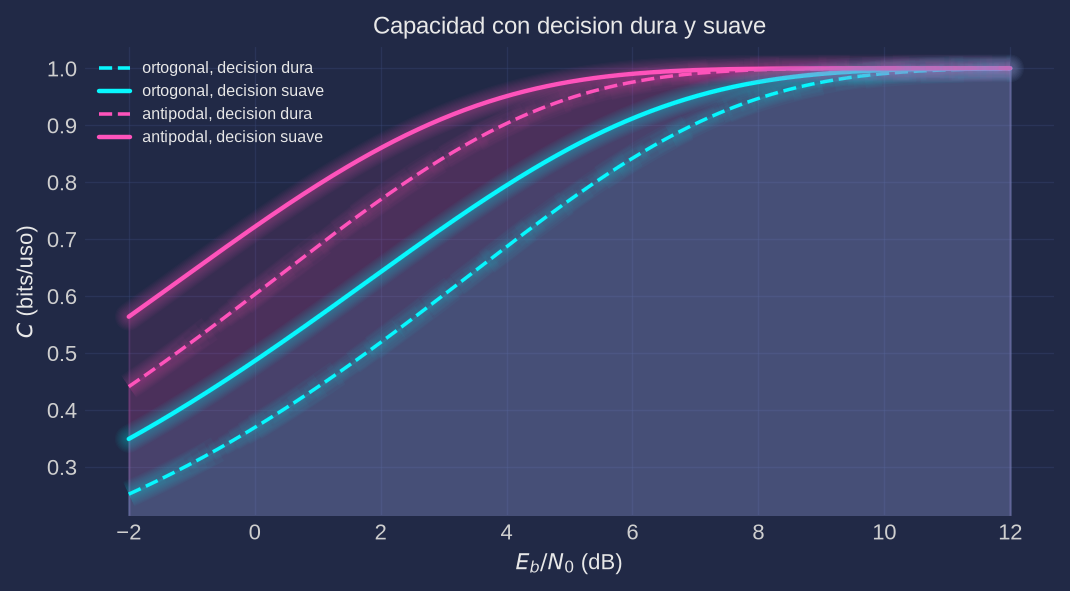
\includegraphics[width=0.9\linewidth]{p08_decisiones.png}
  \caption{Capacidad con decisión dura y suave para señales ortogonales y
  antipodales.}
\end{figure}

\subsection*{Problema 9: detección coherente y no coherente}

Para señalización ortogonal binaria,
\begin{equation}
  P_{e,\text{coh}}=Q\!\left(\sqrt{\frac{E_b}{N_0}}\right),\qquad
  P_{e,\text{nc}}=\frac12 e^{-E_b/(2N_0)}.
\end{equation}
En ambos casos $C=1-H_b(P_e)$. A 10 dB, $C_{\text{coh}}=0.9908$ y
$C_{\text{nc}}=0.9675$. La detección no coherente pierde porque no usa la fase
de la portadora; la diferencia se reduce al aumentar $E_b/N_0$, pero la
coherente siempre va adelante.
\begin{figure}[H]
  \centering
  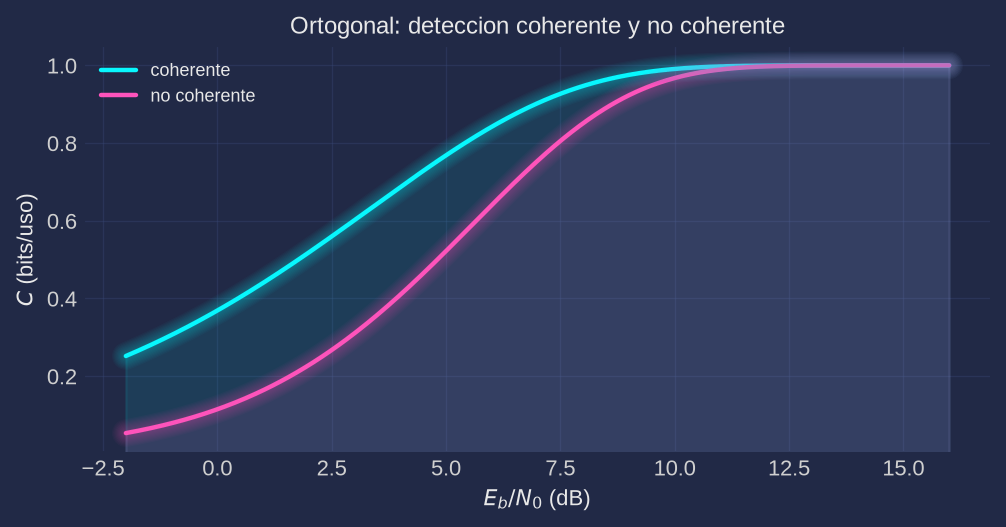
\includegraphics[width=0.85\linewidth]{p09_coherente_no_coherente.png}
  \caption{Capacidad de señalización ortogonal con detección coherente y no
  coherente.}
\end{figure}

% =======================================================================
\section*{2. Códigos de bloque (problemas 10 a 14)}

\subsection*{Problema 10: matriz generadora de Hamming sistemática}

Para cualquier $m\ge 2$, el código de Hamming tiene $n=2^m-1$ y $k=n-m$. Se
construye $H=[A\mid I_m]$, donde las columnas de $A$ son todos los vectores
binarios no nulos de $m$ bits excepto los vectores unitarios; así las columnas
de $H$ son todos los vectores no nulos exactamente una vez. Entonces
$G=[I_k\mid A^T]$ y $GH^T=0$. El script verifica la ortogonalidad para
$m=2,3,4,5$. Las tasas son $1/3$, $4/7$, $11/15$ y $26/31$.
\begin{figure}[H]
  \centering
  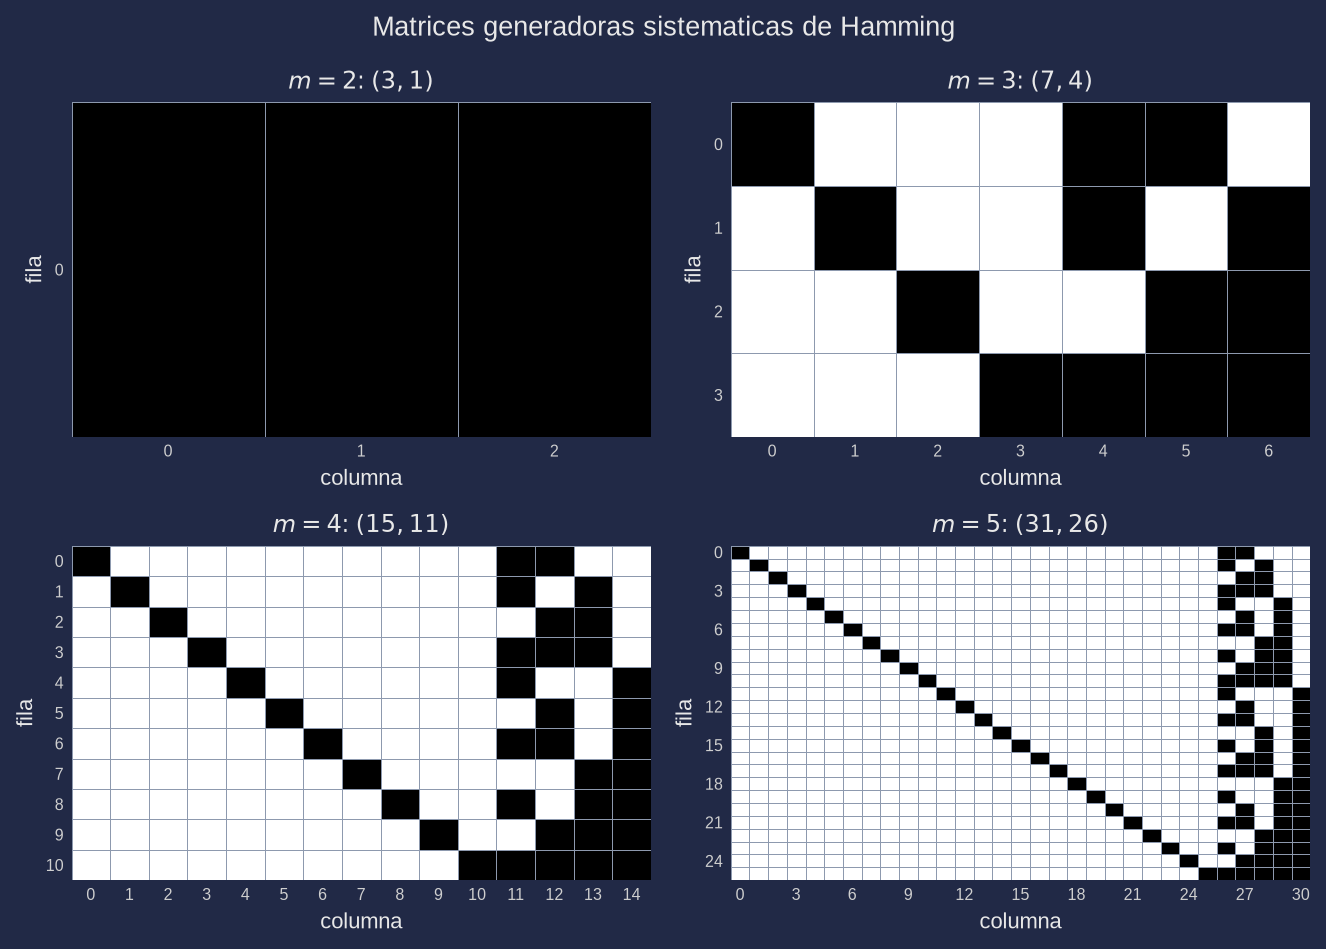
\includegraphics[width=0.95\linewidth]{p10_hamming.png}
  \caption{Matrices generadoras sistemáticas de Hamming para $m=2,3,4,5$.}
\end{figure}
Por ejemplo, para $m=3$:
\begin{equation}
  G=
  \begin{pmatrix}
    1&0&0&0&1&1&0\\
    0&1&0&0&1&0&1\\
    0&0&1&0&0&1&1\\
    0&0&0&1&1&1&1
  \end{pmatrix}.
\end{equation}

\subsection*{Problema 11: Hamming (7,4) con señalización ortogonal}

Se usa el código $(7,4)$, tasa $R=4/7$, con decisión dura y decodificación por
síndrome (líderes de clase lateral). La probabilidad de error por bit después
de decodificar se calcula exactamente enumerando los $2^7$ patrones de error.
Para señalización ortogonal, la probabilidad de error del canal es
$p=Q(\sqrt{RE_b/N_0})$ en coherente y $p=\tfrac12e^{-RE_b/(2N_0)}$ en no
coherente. A 10 dB, $p_{\text{coh}}=0.00841$ y la BER codificada es
$6.22\times10^{-4}$; en no coherente $p=0.02872$ y la BER es
$6.83\times10^{-3}$. La curva sin codificar se incluye para comparar.
\begin{figure}[H]
  \centering
  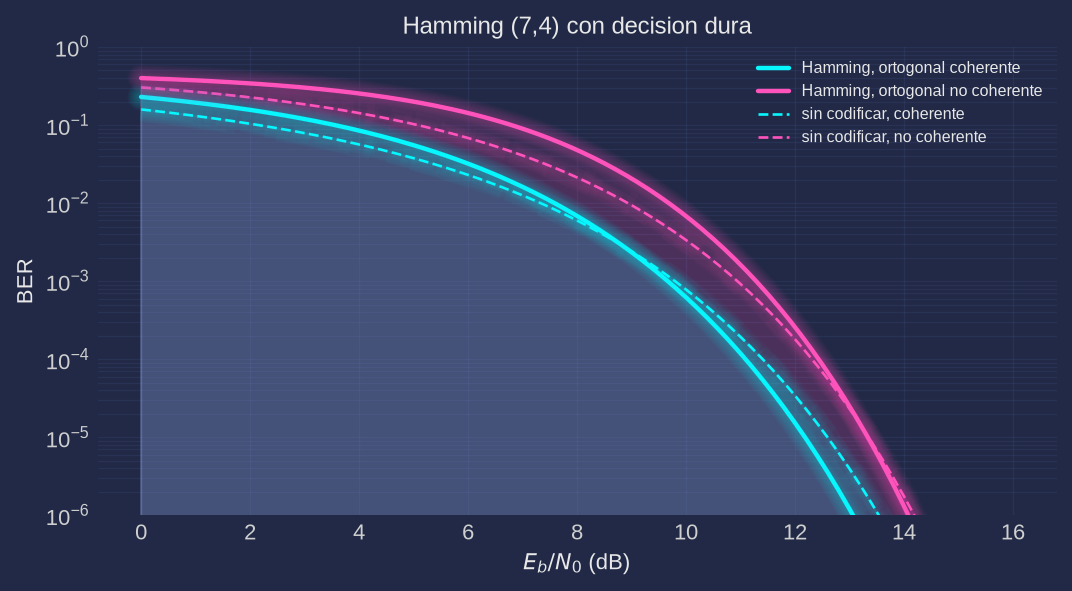
\includegraphics[width=0.9\linewidth]{p11_hamming_ortogonal.png}
  \caption{Hamming $(7,4)$ con decisión dura y señalización ortogonal.}
\end{figure}

\subsection*{Problema 12: Monte Carlo del Hamming con BPSK}

Se simulan 200\,000 bits de información con BPSK, $R=4/7$, ruido AWGN y
decisión dura. La teoría usa el BSC equivalente con
$p=Q(\sqrt{2RE_b/N_0})$. La simulación coincide con la teoría; a 9 dB la BER
medida es $3.5\times10^{-5}$ frente a $1.5\times10^{-5}$ teórica. A 10 dB no se
observaron errores en 200\,000 bits, mientras que la teoría predice
$1.18\times10^{-6}$; el cero es el límite de resolución de la simulación.
\begin{figure}[H]
  \centering
  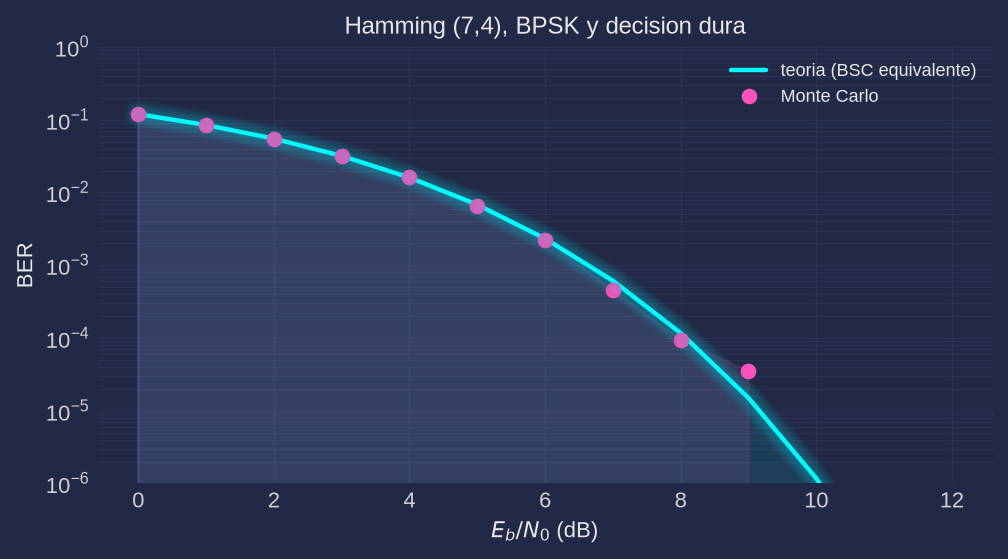
\includegraphics[width=0.85\linewidth]{p12_hamming_mc.png}
  \caption{Monte Carlo del Hamming $(7,4)$ con BPSK y decisión dura.}
\end{figure}

\subsection*{Problema 13: decisión suave con señales ortogonales}

Ahora el decodificador de Hamming usa las LLR de los siete bits y elige la
palabra del código con mayor verosimilitud (16 palabras). Para el canal
ortogonal coherente, la LLR es gaussiana; para el no coherente se usan las
envolventes Rice/Rayleigh y la función de Bessel $I_0$. A 10 dB:
\begin{table}[H]
  \centering
  \begin{tabular}{lcc}
    \toprule
    Decisión & Coherente & No coherente\\
    \midrule
    Dura & $6.22\times10^{-4}$ & $6.83\times10^{-3}$\\
    Suave & $5.0\times10^{-5}$ & $1.79\times10^{-3}$\\
    \bottomrule
  \end{tabular}
  \caption{BER del Hamming $(7,4)$ a $E_b/N_0=10$ dB.}
\end{table}
La decisión suave mejora unas 12 veces en coherente y unas 3.8 veces en no
coherente. La ganancia es mayor en coherente porque la LLR conserva toda la
información de amplitud y fase.
\begin{figure}[H]
  \centering
  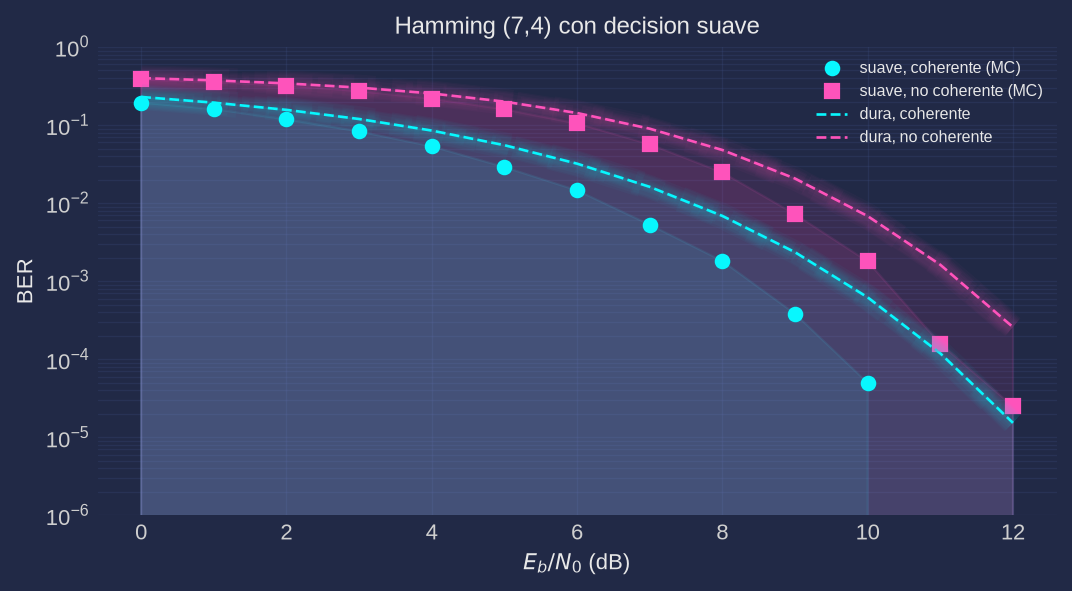
\includegraphics[width=0.9\linewidth]{p13_hamming_suave.png}
  \caption{Hamming $(7,4)$ con decisión suave y señales ortogonales.}
\end{figure}

\subsection*{Problema 14: confirmación Monte Carlo de la decisión suave}

Se repite la simulación con otra semilla y 200\,000 bits por punto. Los
resultados confirman las curvas del problema 13. A 10 dB la BER coherente es
$6\times10^{-5}$ y la no coherente $1.435\times10^{-3}$; a 12 dB son
$0$ y $1.5\times10^{-5}$, respectivamente.
\begin{figure}[H]
  \centering
  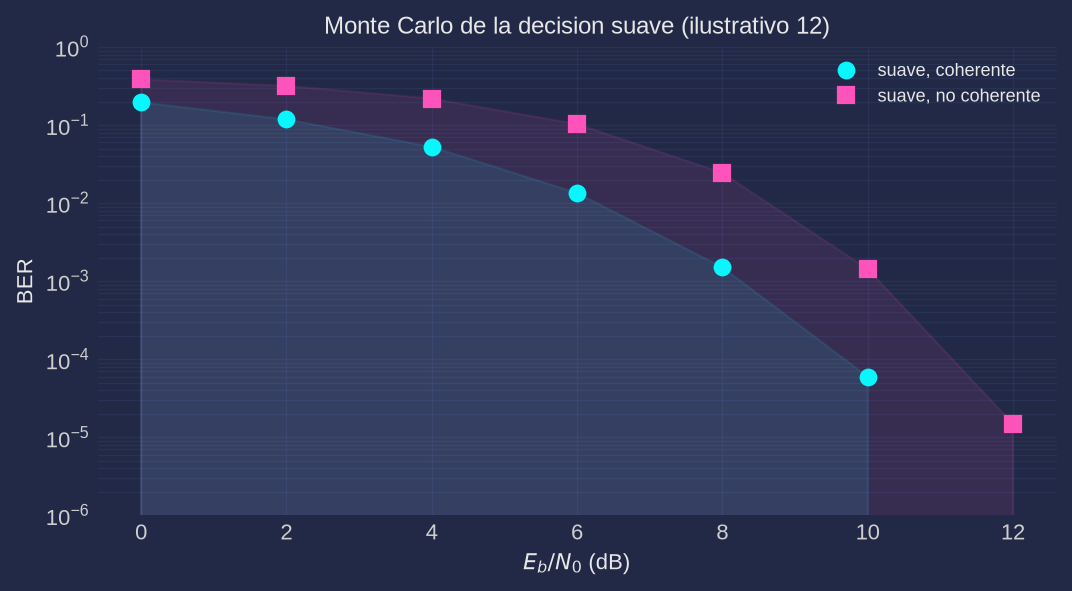
\includegraphics[width=0.85\linewidth]{p14_hamming_suave_mc.png}
  \caption{Monte Carlo independiente de la decisión suave.}
\end{figure}

% =======================================================================
\section*{3. Códigos convolucionales (problemas 15 a 20)}

\subsection*{Problema 15: salida del codificador de la Figura 18}

Se adopta el codificador convolucional de tasa $1/2$, $K=3$, con generadores
$g_1=101_2=5$ y $g_2=111_2=7$. Para la entrada
\texttt{110010101010010111101011111010} (30 bits), la salida es
\begin{center}
\ttfamily
111010111101000100010001111101001001011000010010010101100001
\end{center}
de 60 bits. La figura muestra la entrada y las dos secuencias de salida.
\begin{figure}[H]
  \centering
  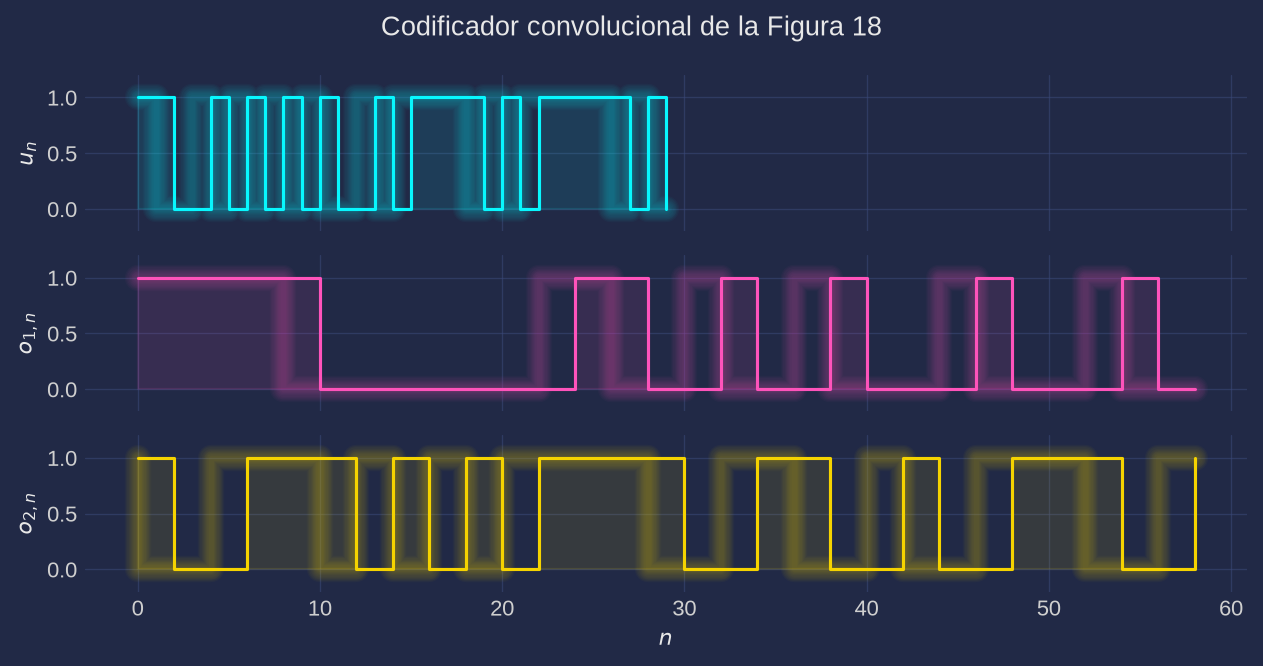
\includegraphics[width=0.9\linewidth]{p15_convolucional.png}
  \caption{Codificador convolucional $(5,7)$ de la Figura 18.}
\end{figure}

\subsection*{Problema 16: código descrito por la matriz $G$}

La matriz del enunciado es
\begin{equation}
  G=
  \begin{pmatrix}
    1&0&1&1\\
    0&1&1&0\\
    1&1&0&1\\
    1&1&1&1
  \end{pmatrix}.
\end{equation}
Para $k=1$ se interpreta como un código de tasa $1/4$ con memoria 3: cada fila
son los coeficientes de retardo $0,1,2,3$ y se obtienen 120 bits de salida para
30 bits de entrada. Para $k=2$ se agrupan las filas en $G_0$ (primeras dos) y
$G_1$ (últimas dos), lo que da un código de tasa $2/4=1/2$ con memoria 1 y 60
bits de salida. Las salidas completas están en \texttt{resultados.json}; la
figura muestra la matriz y las dos secuencias.
\begin{figure}[H]
  \centering
  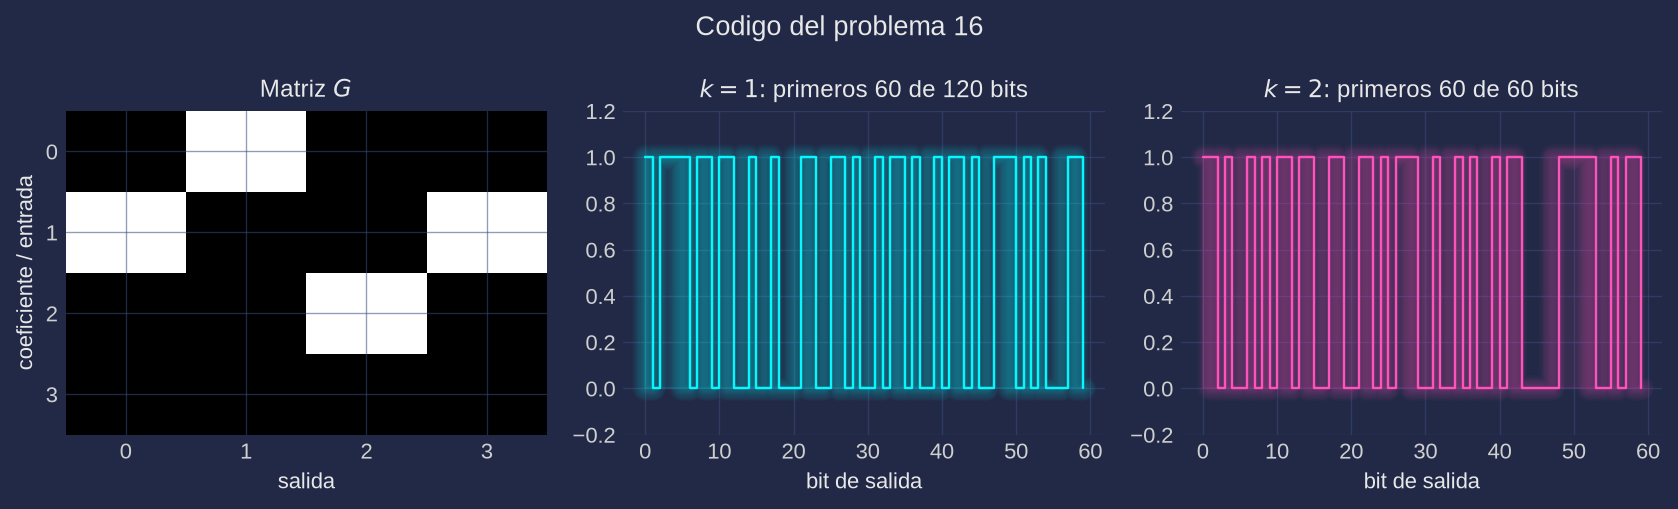
\includegraphics[width=0.95\linewidth]{p16_convolucional_g.png}
  \caption{Matriz $G$ del problema 16 y salidas para $k=1$ y $k=2$.}
\end{figure}

\subsection*{Problema 17: decodificación de Viterbi con errores}

Se codifica la secuencia del problema 15 y se cambian los primeros 6 bits, los
últimos 6, y los primeros 3 más los últimos 3. El decodificador de Viterbi usa
la métrica de Hamming. Los resultados son:
\begin{table}[H]
  \centering
  \begin{tabular}{lcc}
    \toprule
    Caso & Bits erróneos & Métrica final\\
    \midrule
    Sin errores & 0 & 0\\
    Primeros 6 & 1 & 1\\
    Últimos 6 & 1 & 1\\
    3 + 3 & 3 & 4\\
    \bottomrule
  \end{tabular}
  \caption{Errores después de Viterbi para la secuencia de 30 bits.}
\end{table}
El código puede corregir algunos patrones de 6 errores porque la distancia libre
es 5 y los errores están concentrados; cuando se reparten en los dos extremos
el decodificador se equivoca en tres bits.
\begin{figure}[H]
  \centering
  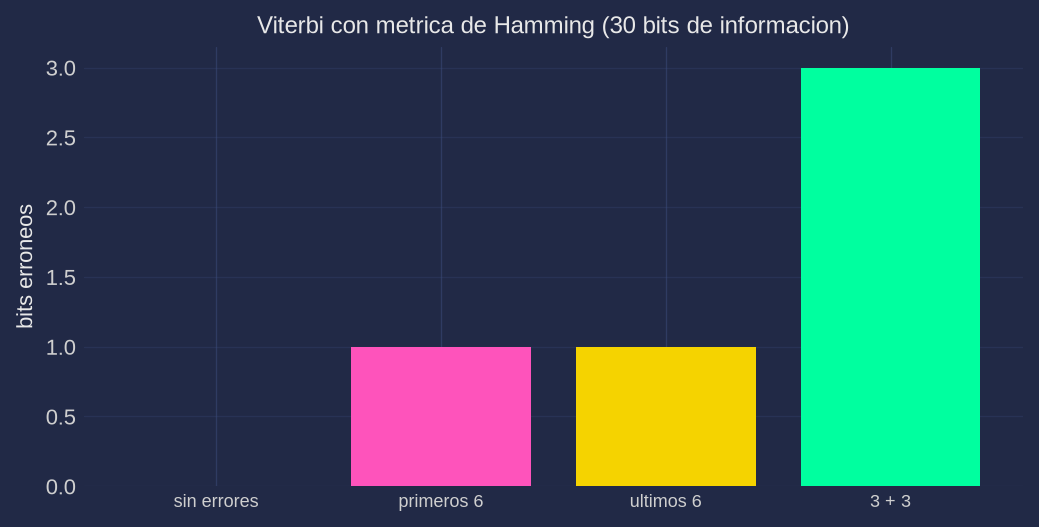
\includegraphics[width=0.8\linewidth]{p17_viterbi.png}
  \caption{Bits erróneos después de Viterbi para los tres patrones.}
\end{figure}

\subsection*{Problema 18: 1000 bits con errores aleatorios}

Se generan 1000 bits equiprobables, se codifican con el código $(5,7)$ y se
suman cuatro secuencias de error de longitud 2000 con probabilidades
$p=0.01,0.05,0.1,0.2$. Se repiten 30 corridas para estimar la BER. Los
resultados medios son:
\begin{table}[H]
  \centering
  \begin{tabular}{lcccc}
    \toprule
    $p$ & 0.01 & 0.05 & 0.10 & 0.20\\
    \midrule
    BER media & $3.3\times10^{-5}$ & $8.1\times10^{-3}$ & $6.89\times10^{-2}$ & $0.2977$\\
    Desviación & $1.8\times10^{-4}$ & $4.4\times10^{-3}$ & $1.95\times10^{-2}$ & $2.60\times10^{-2}$\\
    \bottomrule
  \end{tabular}
  \caption{BER del código convolucional con errores aleatorios.}
\end{table}
El código reduce la BER frente a $p$ para $p\le0.1$; a $p=0.2$ la mejora es
pequeña porque el canal está muy degradado.
\begin{figure}[H]
  \centering
  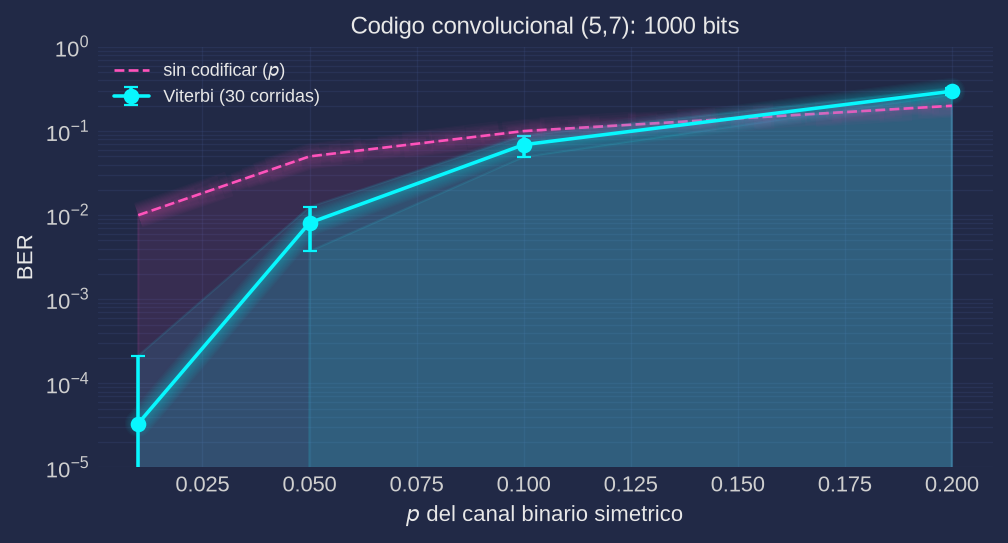
\includegraphics[width=0.82\linewidth]{p18_viterbi_errores.png}
  \caption{BER del código $(5,7)$ contra la probabilidad de error del BSC.}
\end{figure}

\subsection*{Problema 19: BER contra $E_b/N_0$ con decisión dura y suave}

Se simulan 80\,000 bits por punto con BPSK, $R=1/2$ y Viterbi. En decisión dura
se usan bits y métrica de Hamming; en suave se usan las muestras analógicas y
la métrica de correlación. La cota teórica es una unión truncada calculada
enumerando bloques terminados de 14 bits. Los valores en 3, 6 y 9 dB son:
\begin{table}[H]
  \centering
  \begin{tabular}{lccc}
    \toprule
    & 3 dB & 6 dB & 9 dB\\
    \midrule
    Duro (MC) & $3.15\times10^{-2}$ & $8.13\times10^{-4}$ & 0\\
    Suave (MC) & $4.06\times10^{-3}$ & $2.5\times10^{-5}$ & 0\\
    Cota dura & $0.504$ & $8.23\times10^{-4}$ & $8.16\times10^{-6}$\\
    Cota suave & $1.41\times10^{-2}$ & $2.71\times10^{-6}$ & $3.01\times10^{-9}$\\
    \bottomrule
  \end{tabular}
  \caption{BER simulada y cotas truncadas para el código $(5,7)$.}
\end{table}
La decisión suave gana varios dB. Las cotas son superiores a la simulación,
como debe ser; la cota dura es muy holgada a baja SNR porque la unión suma
muchos eventos. Los ceros indican que no se observaron errores en 80\,000 bits.
\begin{figure}[H]
  \centering
  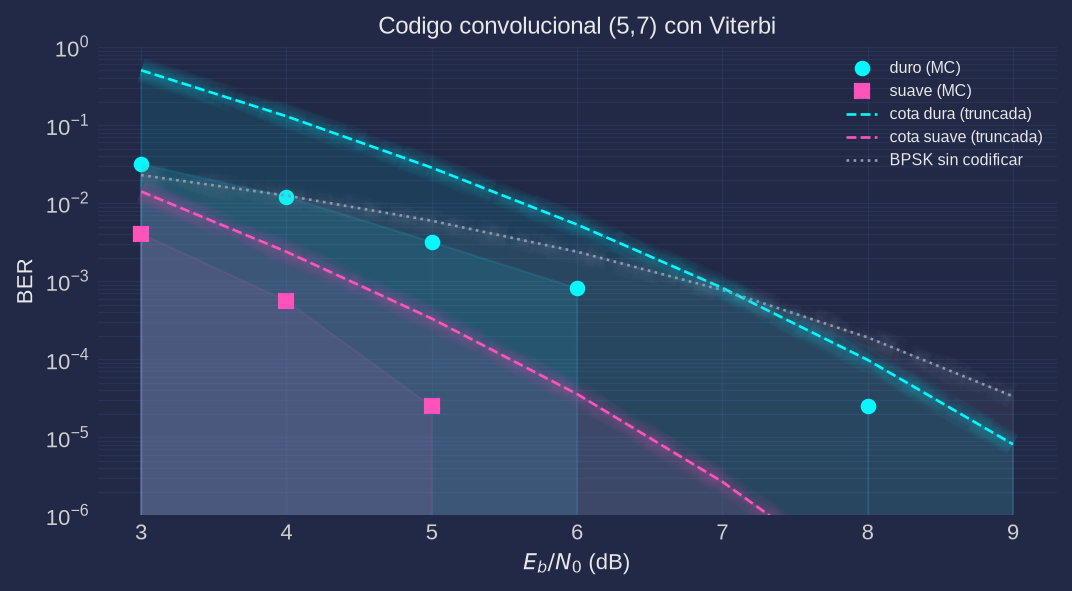
\includegraphics[width=0.9\linewidth]{p19_convolucional_ber.png}
  \caption{BER del código $(5,7)$ con Viterbi y cotas teóricas.}
\end{figure}

\subsection*{Problema 20: Viterbi sobre un canal de 3 salidas}

El canal tiene matriz
\begin{equation}
  P(Y|X)=
  \begin{pmatrix}
    0.90&0.01&0.09\\
    0.01&0.90&0.09
  \end{pmatrix}.
\end{equation}
La secuencia recibida tiene 38 símbolos; como el código es de tasa $1/2$,
corresponden a 19 bits de información. El Viterbi usa la métrica
$-\log P(y|x)$ por cada bit codificado. La secuencia decodificada es
\begin{center}
\ttfamily
0011001101111110011
\end{center}
con métrica final 45.134. La figura muestra la secuencia recibida y la salida
del decodificador.
\begin{figure}[H]
  \centering
  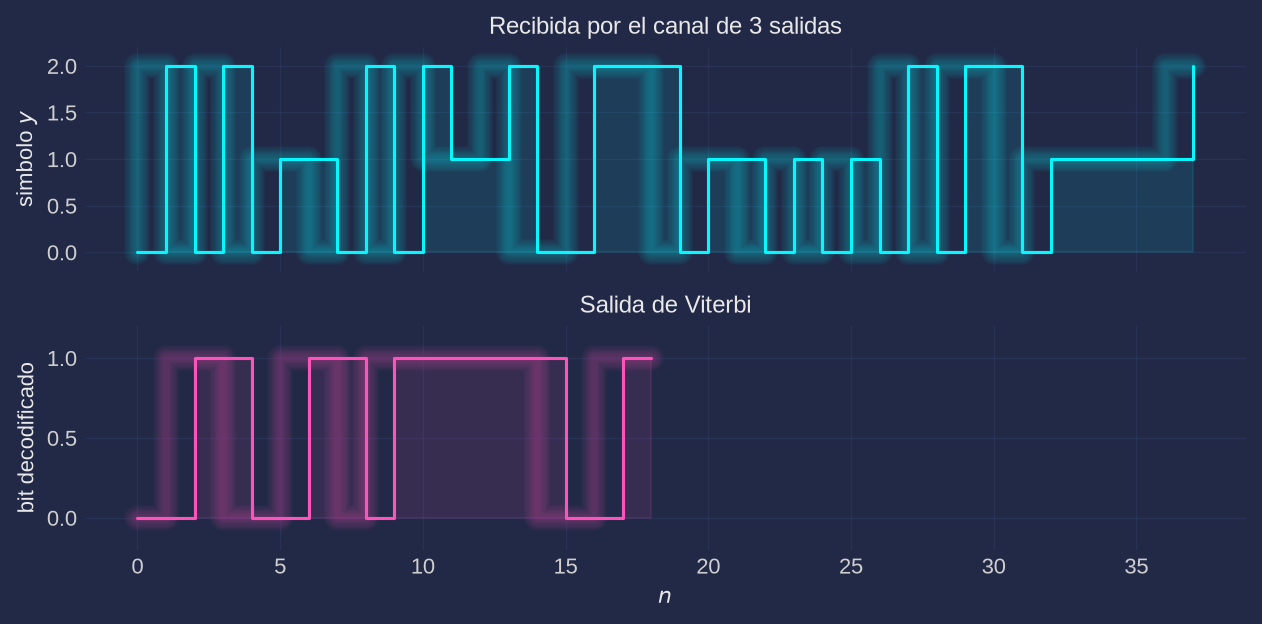
\includegraphics[width=0.85\linewidth]{p20_viterbi_canal.png}
  \caption{Secuencia recibida y salida de Viterbi en el canal de 3 salidas.}
\end{figure}

% =======================================================================
\section*{4. Turbo códigos y LDPC (problemas 21 a 26)}

\subsection*{Problema 21: identidades de la Ecuación (80)}

Las identidades que se verifican son
\begin{align}
  \log(e^a+e^b)&=\max(a,b)+\log\!\left(1+e^{-|a-b|}\right),\\
  \tanh\!\left(\frac{L}{2}\right)&=\frac{e^L-1}{e^L+1},\\
  L_{X_1\oplus X_2}
  &=2\operatorname{atanh}\!\left(\tanh\frac{L_1}{2}\tanh\frac{L_2}{2}\right)
  =\log\frac{1+e^{L_1+L_2}}{e^{L_1}+e^{L_2}}.
\end{align}
La primera es la base de la recursión \emph{log-sum-exp} del BCJR; la segunda
aparece en la actualización de los nodos de verificación; la tercera es la
regla de la LLR para el XOR. Los errores máximos numéricos son
$0$, $2.2\times10^{-16}$ y $9.6\times10^{-13}$, respectivamente.
\begin{figure}[H]
  \centering
  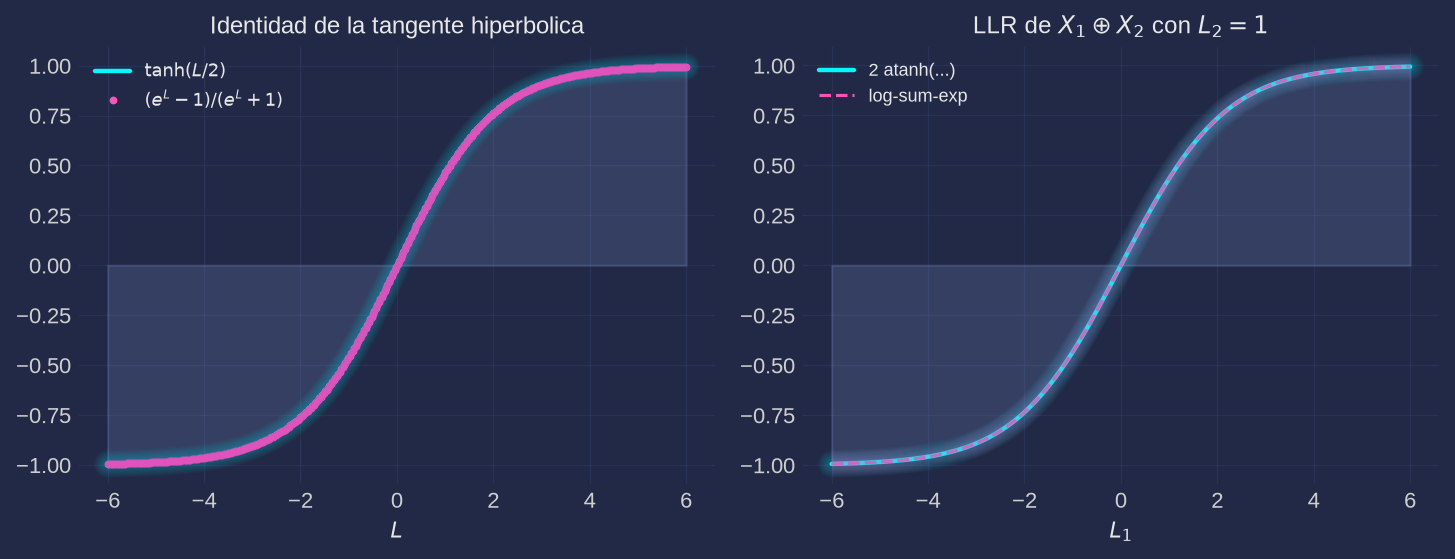
\includegraphics[width=0.95\linewidth]{p21_identidades.png}
  \caption{Verificación numérica de las identidades de la Ecuación (80).}
\end{figure}

\subsection*{Problema 22: entrelazador pseudoaleatorio}

El programa recibe $N$ y devuelve una matriz $2\times N$: el primer renglón es
$1,\dots,N$ y el segundo es una permutación pseudoaleatoria. Para $N=2000$ las
primeras columnas son
\begin{center}
\ttfamily\small
1,2,3,4,5,\dots,20\\
1723,1162,1239,1268,1574,504,1775,1732,1373,1553,1729,428,\\
369,927,954,1924,1538,187,46,284
\end{center}
La permutación se verifica con \texttt{sort}; el desplazamiento medio es 0 y el
máximo es 1959.
\begin{figure}[H]
  \centering
  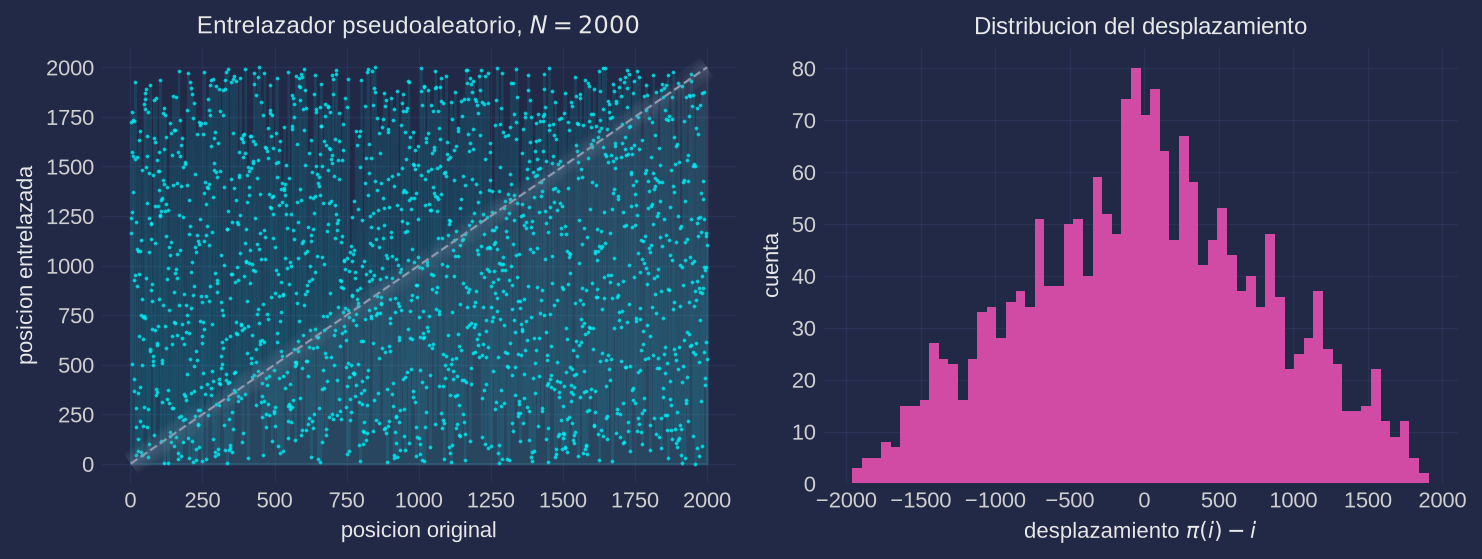
\includegraphics[width=0.95\linewidth]{p22_entrelazador.png}
  \caption{Entrelazador pseudoaleatorio de longitud $N=2000$.}
\end{figure}

\subsection*{Problema 23: turbo codificador RSC (5,7)}

El codificador turbo usa dos RSC de tasa $1/2$ con polinomios $(5,7)$ y un
entrelazador pseudoaleatorio. La salida es la terna $(u,p_1,p_2)$, de tasa
$1/3$ (sin puncturing). Para $N=2000$ y una secuencia pseudoaleatoria, los
primeros 30 bits son
\begin{center}
\ttfamily
u: 111101100011111011011001101001\\
p1: 101110010100000111100100101111\\
p2: 101000111011010000010110101011
\end{center}
\begin{figure}[H]
  \centering
  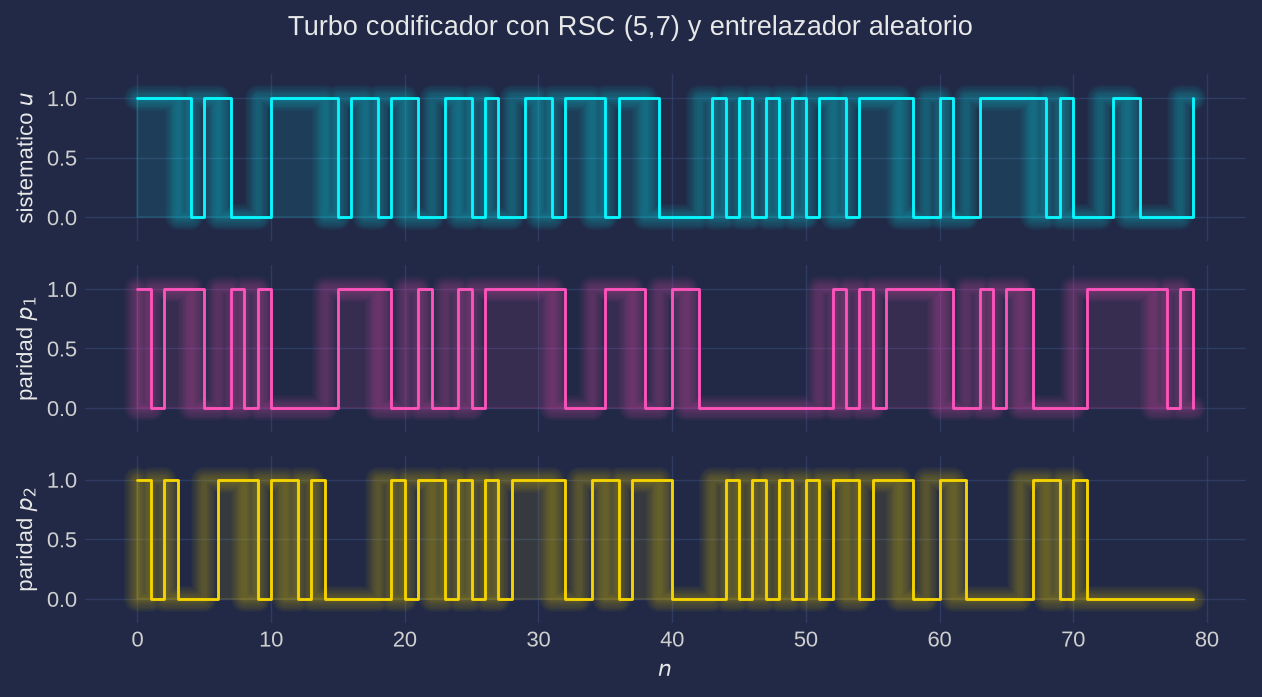
\includegraphics[width=0.9\linewidth]{p23_turbo_encoder.png}
  \caption{Turbo codificador con RSC $(5,7)$ y entrelazador aleatorio.}
\end{figure}

\subsection*{Problema 24: turbo decodificador con BCJR}

Se implementa un decodificador SISO BCJR en el dominio logarítmico y se itera
entre los dos decodificadores, pasando la información extrínseca por el
entrelazador. La simulación usa BPSK, AWGN, $N=500$ y 2500 bits por punto. Los
resultados son:
\begin{table}[H]
  \centering
  \begin{tabular}{lccccc}
    \toprule
    $E_b/N_0$ (dB) & 0 & 1 & 2 & 3 & 4\\
    \midrule
    1 iteración & 0.1640 & 0.1416 & 0.0776 & 0.0356 & 0.0088\\
    5 iteraciones & 0.1004 & 0 & $8\times10^{-4}$ & 0 & 0\\
    \bottomrule
  \end{tabular}
  \caption{BER del turbo decodificador.}
\end{table}
A 2 dB, la BER baja de $6.9\times10^{-2}$ con una iteración a $5\times10^{-3}$
con dos y a cero con tres o más (en 1600 bits). Los ceros significan que no se
observaron errores; la curva no es monótona por el tamaño de la simulación.
\begin{figure}[H]
  \centering
  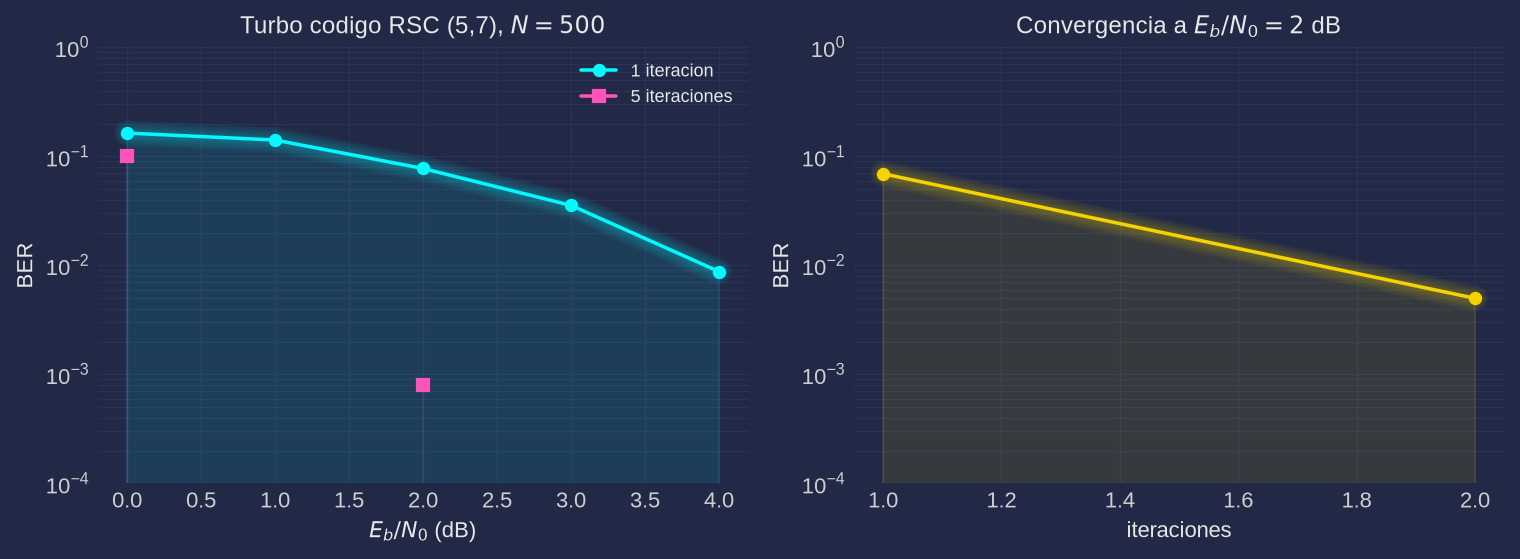
\includegraphics[width=0.95\linewidth]{p24_turbo_decoder.png}
  \caption{BER del turbo código y convergencia con las iteraciones.}
\end{figure}

\subsection*{Problema 25: decodificación por volteo de bit}

La matriz de verificación es
\begin{equation}
  H=
  \begin{pmatrix}
    1&1&0&1&0&0\\
    0&1&1&0&1&0\\
    1&0&0&0&1&1\\
    0&0&1&1&0&1
  \end{pmatrix}.
\end{equation}
Su rango es 3, así que el código es $(6,3)$ y su distancia mínima es 3. El
algoritmo de volteo de bit calcula el síndrome, cuenta los chequeos
insatisfechos de cada bit y voltea el bit con más chequeos insatisfechos. Los
resultados para un BSC son:
\begin{table}[H]
  \centering
  \begin{tabular}{lcccccc}
    \toprule
    $p$ & 0.01 & 0.02 & 0.05 & 0.08 & 0.10 & 0.15\\
    \midrule
    BER & $5.8\times10^{-4}$ & $3.08\times10^{-3}$ & $1.63\times10^{-2}$ & $3.75\times10^{-2}$ & $5.60\times10^{-2}$ & $0.1110$\\
    \bottomrule
  \end{tabular}
  \caption{BER del volteo de bit para el código $(6,3)$.}
\end{table}
El código mejora al canal sin codificar para $p\ge0.05$; a $p=0.01$ la BER es
muy baja porque casi todos los bloques no tienen errores.
\begin{figure}[H]
  \centering
  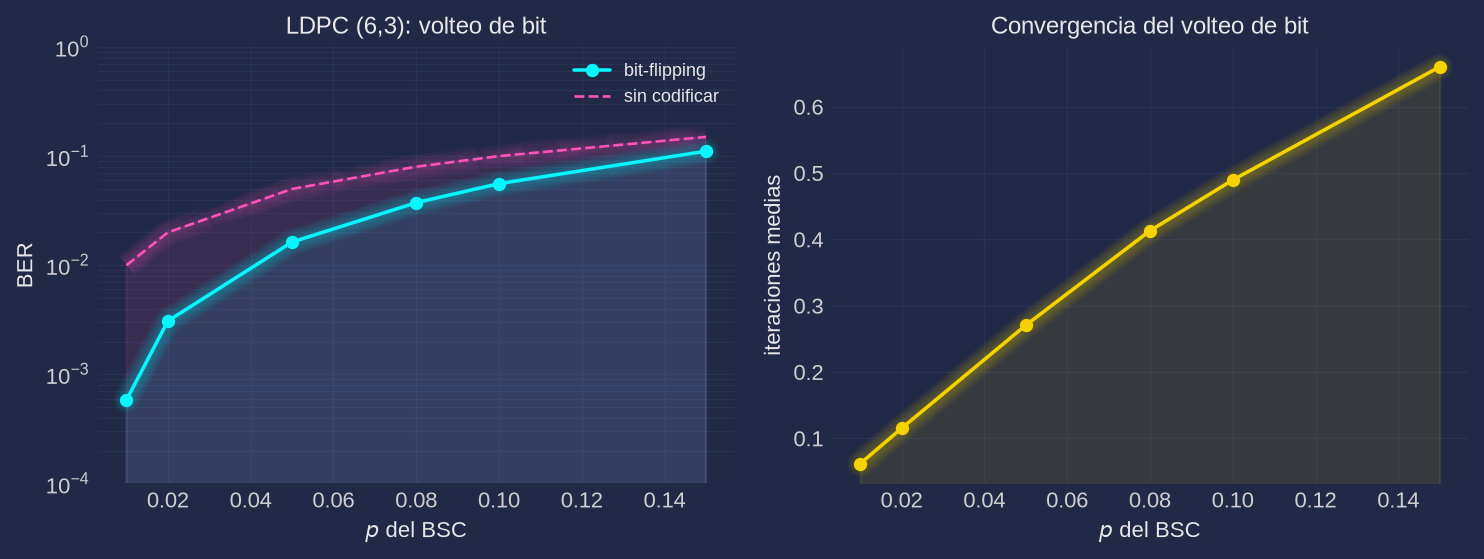
\includegraphics[width=0.95\linewidth]{p25_bit_flipping.png}
  \caption{Volteo de bit para el código LDPC $(6,3)$.}
\end{figure}

\subsection*{Problema 26: decodificación suma-producto}

Se implementa el algoritmo suma-producto en el dominio de las LLR. En cada
nodo de verificación se usa
\begin{equation}
  M_{c\to v}=2\operatorname{atanh}\!\left(\prod_{v'\ne v}
  \tanh\frac{M_{v'\to c}}{2}\right),
\end{equation}
y en cada nodo de variable
\begin{equation}
  M_{v\to c}=L_v+\sum_{c'\ne c}M_{c'\to v}.
\end{equation}
La decisión es $\hat b_v=0$ si la LLR posterior es positiva. La BER contra
$E_b/N_0$ para el código $(6,3)$ es:
\begin{table}[H]
  \centering
  \begin{tabular}{lccccccc}
    \toprule
    $E_b/N_0$ (dB) & 0 & 1 & 2 & 3 & 4 & 5 & 6\\
    \midrule
    Suma-producto & 0.0796 & 0.0531 & 0.0303 & 0.0176 & 0.00614 & 0.00256 & $6.94\times10^{-4}$\\
    Volteo de bit & 0.1211 & 0.0886 & 0.0597 & 0.0397 & 0.0199 & 0.00869 & $2.92\times10^{-3}$\\
    Sin codificar & 0.1585 & 0.1329 & 0.1065 & 0.0804 & 0.0579 & 0.0384 & 0.0229\\
    \bottomrule
  \end{tabular}
  \caption{BER del código $(6,3)$ con suma-producto y volteo de bit.}
\end{table}
La suma-producto supera al volteo de bit porque usa información blanda. La
convergencia con las iteraciones es limitada: el código tiene $d_{\min}=3$ y,
cuando el vector recibido está más cerca de otra palabra, el decodificador
converge a una palabra válida pero errónea. Aun así, la BER baja de
$1.97\times10^{-2}$ con una iteración a $1.52\times10^{-2}$ con diez.
\begin{figure}[H]
  \centering
  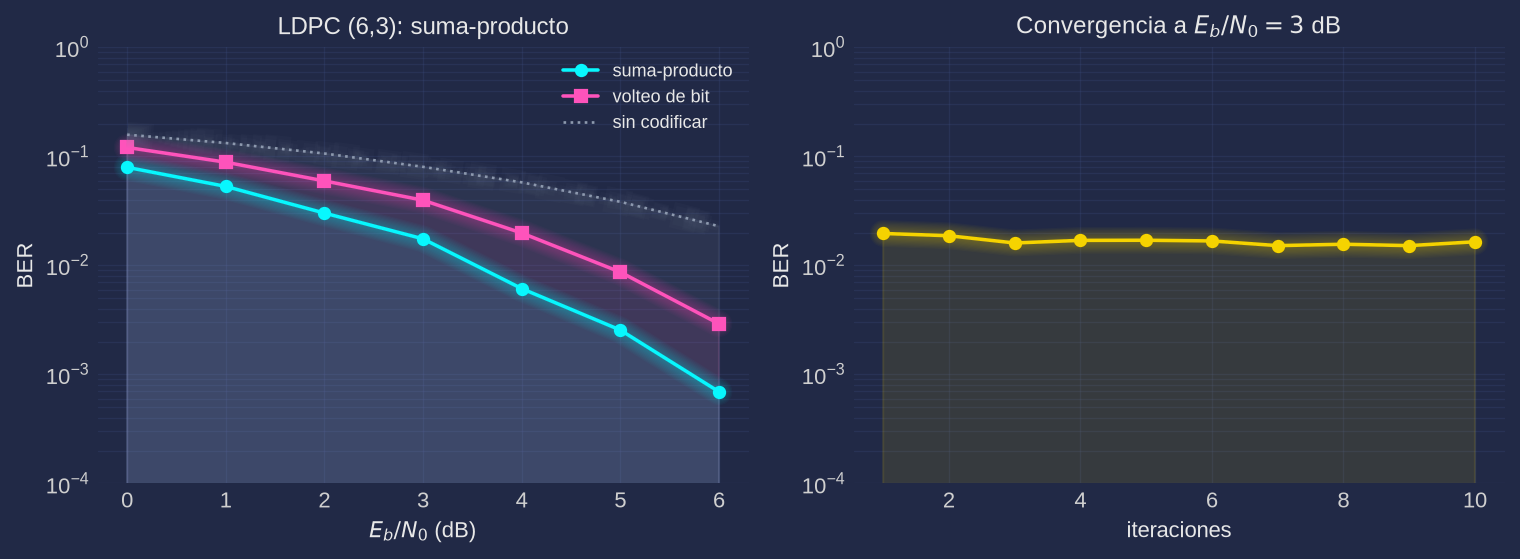
\includegraphics[width=0.95\linewidth]{p26_sum_product.png}
  \caption{Suma-producto para el código LDPC $(6,3)$.}
\end{figure}

% =======================================================================
\section*{Conclusiones}

\begin{itemize}
  \item La capacidad del BSC se anula en $p=1/2$ y es 1 en los extremos. Los
  canales asimétricos y con salidas múltiples tienen distribuciones óptimas de
  entrada que no son uniformes.
  \item La señalización antipodal aprovecha mejor la energía que la ortogonal:
  para la misma $E_b$ la ortogonal está 3 dB peor. La decisión suave y la
  detección coherente también mejoran la capacidad.
  \item El código de Hamming $(7,4)$ reduce la BER en los canales binarios y
  ortogonales; la decisión suave mejora aún más porque conserva la información
  analógica. El Monte Carlo coincide con la teoría.
  \item El código convolucional $(5,7)$ con Viterbi corrige errores y la
  decisión suave gana varios dB frente a la dura. Las cotas de unión truncadas
  son consistentes con la simulación.
  \item El turbo código con RSC $(5,7)$ y BCJR converge en pocas iteraciones;
  el decodificador SISO es la pieza central. El código LDPC $(6,3)$ es pequeño
  y su distancia mínima limita la ganancia, pero el suma-producto supera al
  volteo de bit.
\end{itemize}

% ------------------------------------------------------------------ codigo
\appendix
\section*{Código}
El código completo está en \texttt{tarea2.py} (unas 1500 líneas). Por su extensión
no se incluye en el PDF; el script es autocontenido y regenera todas las
figuras y \texttt{datos/resultados.json} con \texttt{python3 tarea2.py}. Las
funciones están separadas por problema y las secciones principales son:
capacidad (problemas 1 a 9), Hamming y Monte Carlo (10 a 14), convolucionales
y Viterbi (15 a 20), identidades y entrelazador (21 a 23), BCJR y turbo (24),
y LDPC con volteo de bit y suma-producto (25 y 26).

\end{document}
